%%%%%%%%%%%%%%%%%%%%%%%%%%%%%%%%%%%%%%%%%%%%%%%%%%%%%%%%%%%%%%%
%
% Welcome to writeLaTeX --- just edit your LaTeX on the left,
% and we'll compile it for you on the right. If you give
% someone the link to this page, they can edit at the same
% time. See the help menu above for more info. Enjoy!
%
%%%%%%%%%%%%%%%%%%%%%%%%%%%%%%%%%%%%%%%%%%%%%%%%%%%%%%%%%%%%%%%

% --------------------------------------------------------------
% This is all preamble stuff that you don't have to worry about.
% Head down to where it says "Start here"
% --------------------------------------------------------------
 
\documentclass[12pt]{article}
 
\usepackage[margin=1in]{geometry}
\usepackage{amsmath,amsthm,amssymb}

\usepackage{listings}
\usepackage{xcolor}
\usepackage{circuitikz}
\usetikzlibrary{bending}
\usetikzlibrary{patterns,decorations.pathmorphing,positioning}

%New colors defined below
\definecolor{codegreen}{rgb}{0,0.6,0}
\definecolor{codegray}{rgb}{0.5,0.5,0.5}
\definecolor{codepurple}{rgb}{0.58,0,0.82}
\definecolor{backcolour}{rgb}{0.95,0.95,0.92}

%Code listing style named "mystyle"
\lstdefinestyle{mystyle}{
  backgroundcolor=\color{backcolour}, commentstyle=\color{codegreen},
  keywordstyle=\color{magenta},
  numberstyle=\tiny\color{codegray},
  stringstyle=\color{codepurple},
  basicstyle=\ttfamily\footnotesize,
  breakatwhitespace=false,         
  breaklines=true,                 
  captionpos=b,                    
  keepspaces=true,                 
  numbers=left,                    
  numbersep=5pt,                  
  showspaces=false,                
  showstringspaces=false,
  showtabs=false,                  
  tabsize=2
}

%"mystyle" code listing set
\lstset{style=mystyle}

 
\newcommand{\N}{\mathbb{N}}
\newcommand{\Z}{\mathbb{Z}}
 
\newenvironment{theorem}[2][Theorem]{\begin{trivlist}
\item[\hskip \labelsep {\bfseries #1}\hskip \labelsep {\bfseries #2.}]}{\end{trivlist}}
\newenvironment{lemma}[2][Lemma]{\begin{trivlist}
\item[\hskip \labelsep {\bfseries #1}\hskip \labelsep {\bfseries #2.}]}{\end{trivlist}}
\newenvironment{exercise}[2][Exercise]{\begin{trivlist}
\item[\hskip \labelsep {\bfseries #1}\hskip \labelsep {\bfseries #2.}]}{\end{trivlist}}
\newenvironment{problem}[2][Problem]{\begin{trivlist}
\item[\hskip \labelsep {\bfseries #1}\hskip \labelsep {\bfseries #2.}]}{\end{trivlist}}
\newenvironment{question}[2][Question]{\begin{trivlist}
\item[\hskip \labelsep {\bfseries #1}\hskip \labelsep {\bfseries #2.}]}{\end{trivlist}}
\newenvironment{corollary}[2][Corollary]{\begin{trivlist}
\item[\hskip \labelsep {\bfseries #1}\hskip \labelsep {\bfseries #2.}]}{\end{trivlist}}

\newenvironment{solution}{\begin{proof}[Solution]}{\end{proof}}
 
\begin{document}
 
% --------------------------------------------------------------
%                         Start here
% --------------------------------------------------------------
 
\title{Homework 1}%replace X with the appropriate number
\author{Mengxiang Jiang\\ %replace with your name
EEEN 5338 Digital and DSP Based Control} %if necessary, replace with your course title
 
\maketitle
 
\begin{problem}{1} %You can use theorem, exercise, problem, or question here.  Modify x.yz to be whatever number you are proving
Find the math model for the following system. Assume: $R_1=R_2=R_3=R_4=1\Omega$.
\\
\begin{circuitikz} \draw
  (0,4) to[battery, l=$x(t)$] (0,0) -- (4,0)
  to [resistor, l=$R_2$] (4,4)
  to [resistor, l=$R_1$] (0,4)
  (12,4) to [battery, l=$y(t)$] (12,0) -- (4,0)
  (12,4) -- (8,4) 
  to [resistor, l=$R_3$] (4,4)
  (8,4) to [resistor, l=$R_4$] (8,0);
  \draw[thin, <-] (2,2)node{$i_1$}  ++(-45:1) arc (-45:135:1);
  \draw[thin, <-] (6,2)node{$i_2$}  ++(-45:1) arc (-45:135:1);

\end{circuitikz}
\begin{equation}
  x=R_1i_1+R_2(i_1-i_2) = 2i_1-i_2
\end{equation}
\begin{equation}
  R_2(i_2-i_1)+R_3i_2+R_4i_2 = 3i_2-i_1=0 \implies 3i_2=i_1
\end{equation}
\begin{equation}
  y=R_4i_2=i_2
\end{equation}
If we put everything in terms of $i_2$, we have $x=5i_2$ and since $y=i_2$, $x=5y$.
\end{problem}
\pagebreak
\begin{problem}{2}
Find the math model for the following system. Assume: $R_1=R_2=1\Omega$, $L=1H$, $C=1F$.
\\
\begin{circuitikz} \draw
  (0,4) to[battery, l=$x(t)$] (0,0) -- (4,0)
  to [resistor, l=$R_1$] (4,4)
  to [inductor, l=$L$] (0,4)
  (12,4) to [battery, l=$y(t)$] (12,0) -- (4,0)
  (12,4) -- (8,4) 
  to [resistor, l=$R_2$] (4,4)
  (8,4) to [capacitor, l=$C$] (8,0);
  \draw[thin, <-] (2,2)node{$i_1$}  ++(-45:1) arc (-45:135:1);
  \draw[thin, <-] (6,2)node{$i_2$}  ++(-45:1) arc (-45:135:1);

\end{circuitikz}
\begin{equation}
  x=L\frac{di_1}{dt} + R_1(i_1-i_2) = \frac{di_1}{dt} + i_1 - i_2
\end{equation}
\begin{equation}
  \begin{split}
  R_1(i_2-i_1)+R_2i_2+\frac{1}{C}\int{i_2dt}=0 \\
  \implies \frac{2di_2}{dt} - \frac{di_1}{dt} + i_2 = 0\\
  \implies \frac{di_1}{dt} = \frac{2di_2}{dt} + i_2
  \end{split}
\end{equation}
\begin{equation}
  \begin{split}
  y=\frac{1}{C}\int{i_2dt}\\
  \implies \dot{y} = i_2
  \end{split}
\end{equation}
Using (5) and (6), we have\\
\begin{equation}
  \frac{di_1}{dt} = 2\ddot{y} + \dot{y}
\end{equation} 
Taking the derivative of (4) and substituting in the results from (6) and (7), we have\\
\begin{equation}
  \begin{split}
  \dot{x} = \frac{d^2i_1}{dt^2} + \frac{di_1}{dt} - \frac{di_2}{dt}\\
  \implies \dot{x} = 2\dddot{y} +\ddot{y} + 2\ddot{y}+\dot{y} - \ddot{y}= 2\dddot{y}+2\ddot{y}+\dot{y}\\
  \implies x = 2\ddot{y} +2\dot{y} + y
  \end{split}
\end{equation}
\end{problem}
\pagebreak
\begin{problem}{2}
  Find the math model for the following system. (Note: \LaTeX \space doesn't have a good way of drawing rotational mechanical systems, so I am drawing an equivalent translational one instead).\\
  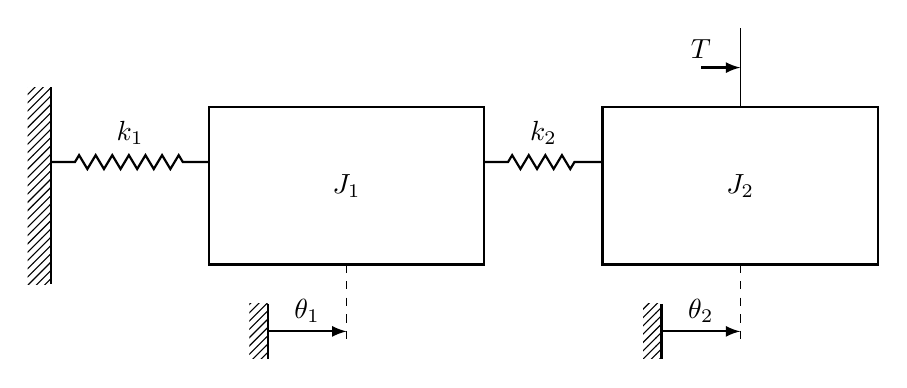
\begin{tikzpicture}[every node/.style={outer sep=0pt},thick,
    mass/.style={draw,thick},
    spring/.style={thick,decorate,decoration={zigzag,pre length=0.3cm,post
    length=0.3cm,segment length=6}},
    ground/.style={fill,pattern=north east lines,draw=none,minimum
    width=0.75cm,minimum height=0.3cm},
    dampic/.pic={\fill[white] (-0.1,-0.3) rectangle (0.3,0.3);
    \draw (-0.3,0.3) -| (0.3,-0.3) -- (-0.3,-0.3);
    \draw[line width=1mm] (-0.1,-0.3) -- (-0.1,0.3);}]
   
     \node[mass,minimum width=3.5cm,minimum height=2cm] (m1) {$J_1$};
     \node[mass,minimum width=3.5cm,minimum height=2cm,right=1.5cm of
     m1] (m2) {$J_2$};
     \node[left=2cm of m1,ground,minimum width=3mm,minimum height=2.5cm] (g1){};
     \draw (g1.north east) -- (g1.south east);
   
     \draw[spring] ([yshift=3mm]g1.east) coordinate(aux)
      -- (m1.west|-aux) node[midway,above=1mm]{$k_1$};
     \draw[spring]  (m1.east|-aux) -- (m2.west|-aux) node[midway,above=1mm]{$k_2$};
   
     \foreach \X in {1,2}  
     {
      \draw[thin,dashed] (m\X.south) -- ++ (0,-1) coordinate[pos=0.85](aux'\X);
      \draw[latex-] (aux'\X) -- ++ (-1,0) node[midway,above]{$\theta_\X$}
       node[left,ground,minimum height=7mm,minimum width=1mm] (g'\X){};
      \draw[thick] (g'\X.north east) -- (g'\X.south east);
     }
     \draw[thin] (m2.north) -- ++ (0,1) coordinate[midway](aux2);
     \draw[latex-] (aux2) -- ++ (-0.5,0) node[above]{$T$}; 
   \end{tikzpicture}

   \begin{equation}
    \begin{split}
      \sum{T} = J\alpha\\
      -k_1\theta_1+k_2(\theta_2-\theta_1)=J_1\ddot{\theta_1}\\
      -k_2(\theta_2-\theta_1)+T=J_2\ddot{\theta_2}\\
      J_1\ddot{\theta_1} + (k_1+k_2)\theta_1 - k_2\theta_2 = 0\\
      J_2\ddot{\theta_2} - k_2\theta_1 + k_2\theta_2 = T\\
    \end{split}
   \end{equation}

\end{problem}
% --------------------------------------------------------------
%     You don't have to mess with anything below this line.
% --------------------------------------------------------------
 
\end{document}